\chapter{Interaction matière-lumière}
\section{Équations de Maxwell}
Les équations de \textsc{Maxwell} du champ électrique et du champ d'induction magnétique sont 
désormais bien connue
\begin{equation}
{\bf E} ({\bf r},t) = - \mbox{\boldmath $ \nabla $} \Phi({\bf r},t) - 
  \frac{\partial }{\partial t} {\bf A} ({\bf r},t),\qquad\qquad
  {\bf B} ({\bf r},t) = \mbox{\boldmath $ \nabla $} \times {\bf A} ({\bf r},t)
\end{equation}
La jauge de \textsc{Coulomb} $\vec\nabla.\vec{A}=0$ permet d'imposer des ondes transverses. On obtient
alors l'équation d'onde
\begin{equation}
\nabla ^2 {\bf A} - \frac{1}{c^2} \frac{\partial ^2 {\bf A}}{\partial t ^2} = 0 
\end{equation}
Nous avons en effet $\phi=0$ dans le vide. La solution de cette équation est une onde plane
monochromatique
\begin{equation}
{\bf A}(\omega; {\bf r},t) = {\bf A}_0(\omega) 
   \cos ( {\bf k} \cdot {\bf r} - \omega t  
 + \delta_{\omega} ) 
\end{equation}
où $\vec A_0$ est le vecteur d'amplitude, qui décrit l'intensité et la polarisation de la radiation, $\vec{k}$ est le vecteur de 
propagation ($\omega=kc$) et où $\delta_\omega$ est une phase réelle. Comme annoncé, la jauge de
\textsc{Coulomb} impose
\begin{equation}
\mbox{\boldmath $ \nabla $} \cdot {\bf A} = 0  \; \; \mbox{si} \; \; 
   {\bf k} \cdot {\bf A}_0(\omega) = 0 
\end{equation}
Les ondes sont donc transverses : $\vec{k}\perp\vec{A_0}(\omega)$. Avec ce choix de potentiel vecteur,
nous pouvons ré-écrire le champ électrique, l'induction magnétique 
\begin{equation}
{\bf E} ({\bf r},t)  = E_0(\omega)
\hat{ \mbox{\boldmath $ \epsilon $} } 
  \; \sin ( {\bf k} \cdot {\bf r} - \omega t + \delta_{\omega}),\qquad\qquad
  {\bf B} ({\bf r},t) = E_0(\omega)
\omega^{-1}
 ({\bf k} \times \hat{ \mbox{\boldmath $ \epsilon $}} )
\; \sin ( {\bf k} \cdot {\bf r} - \omega t + \delta_{\omega})
\end{equation}
et le potentiel vecteur
\begin{equation}
 {\bf A}_0(\omega) = A_0(\omega) 
\hat{  \mbox{\boldmath $ \epsilon $}}
\Rightarrow   {\bf k} \cdot 
\hat{  \mbox{\boldmath $ \epsilon $}} = 0
\end{equation}
où $\vec{\hat{\epsilon}}$ est le vecteur de polarisation. Il nous informe la direction dans laquelle
$\vec{A_0}$ pointe. Comme $\vec{E}$ contient également ce vecteur, il est forcément colinéaire à 
$\vec{A_0}$. L'onde est forcément transverse ($\vec{k}\perp\vec{A}$) et la direction de polarisation
de $\vec{E}$ est imposée par $\vec{A}$. Notons qu'il est possible de déterminer un état arbitraire
de polarisation en effectuant la combinaison de deux ondes planes indépendantes. Notons également
que $E_0(\omega) = - \omega A_0(\omega)$.\\

A l'aide du vecteur de \textsc{Poynting} ($\propto |E|^2$), il est possible de déterminer l'intensité
du champ électrique (ou du potentiel vecteur)
\begin{equation}
  I(\omega) 
= \frac{1}{2} \epsilon_0 c E_0^2 (\omega) 
=  \frac{1}{2} \epsilon_0 c \omega^2  A_0^2 (\omega) 
= \frac{\hbar \omega N(\omega) c}{V}
= \rho (\omega) c
\end{equation}
La dernière égalité est le produit de la densité photonique par la vitesse de la lumière. La densité
photonique (ou densité de radiation) s'exprime
\begin{equation}
\rho(\omega) 
= \frac{1}{2} \epsilon_0 E_0^2 (\omega)
= \frac{1}{2} \epsilon_0 \omega^2
A_0^2 (\omega) = \frac{N (\omega) \hbar \omega}{V}
\end{equation}
Cette densité est l'énergie $\hbar\omega$ que porte chaque photon, multiplié par $N(\omega)$ le nombre
de photon, par la vitesse de la lumière $c$ et divisé par le volume. Il s'agit bien d'une énergie par
unité de surface et de temps.\\

Notons les deux relations intégrales suivantes
\begin{equation}
I = \int_0^\infty I (\omega) d\omega \hspace*{1cm};
\hspace*{1cm}
\rho = \int_0^\infty \rho (\omega) d\omega 
\end{equation}
Ces relations sont rencontrée lorsque l'on ne se situe pas dans un cas monochromatique : par exemple,
un \textit{pulse} a une forme dans l'espace et le temps.

\section{Équation de Schrödinger dépendante du temps}
Les solutions des équations de \textsc{Maxwell} pouvant bien évidemment dépendre du temps, il faut se
soucier de l'évolution dans le temps (mais aussi toujours de l'espace) du potentiel vecteur en tenant
compte du fait que ce n'est pas intégralement monochromatique. On défini alors la forme générale d'un
pulse de radiation
\begin{equation}
  {\bf A} ({\bf r}, t) 
= \hat{  \mbox{\boldmath $ \epsilon $}}
\int_{\Delta \omega} A_0 (\omega) 
   \cos ( {\bf k} \cdot {\bf r} - \omega t + 
\delta_{\omega} )  \; d \omega
\end{equation}
L'hamiltonien d'une particule chargée (sans spin) dans un champ électromagnétique s'écrit
\begin{equation}
H = \frac{1}{2m} ({\bf p} - q {\bf A} ) ^2 + q \Phi
\end{equation}
Utilisons celui-ci pour écrire l'équation de Schrödinger dépendante du temps
\begin{equation}
i \hbar \frac{\partial}{\partial t} \Psi ({\bf r}, t)
= \left[ \frac{1}{2m} (-i \hbar  \mbox{\boldmath $ \nabla $} + e {\bf A}) ^2
  - \frac{Ze^2}{(4 \pi \epsilon_0) r } \right] \Psi ({\bf r}, t)
\end{equation}
Comme $\vec\grad A=0$ (jauge de \textsc{Coulomb}), nous avons que
\begin{equation}
 \mbox{\boldmath $ \nabla $} \cdot ({\bf A} \Psi )
= {\bf A} \cdot (  \mbox{\boldmath $ \nabla $} \Psi)
\end{equation}
Il est donc possible de remplacer le double produit par l'un de ces deux termes. A un facteur 2 près,
ça n'a pas d'importance. Ce facteur disparait d'ailleurs dans la forme réécrite ci-dessous
\begin{equation}
i \hbar \frac{\partial}{\partial t} \Psi ({\bf r}, t) =\left[ -\frac{\hbar ^2}{2m} \nabla ^2 - \frac{Ze^2}{(4 \pi \epsilon_0) r } 
  - \underbrace{\frac{i \hbar e}{m} {\bf A} \cdot \mbox{\boldmath $ \nabla $} 
  + \frac{e^2}{2m} {\bf A} ^2}_{(*)} \right] \Psi ({\bf r}, t)
\end{equation}
La ré-écriture fait apparaitre deux termes (marqués par $(*)$) dans l'Hamiltonien. Ceux-ci sont 
négligeable, il est nécessaire que l'intensité soit faible (car $I = f(\vec{A})$).\\

On peut considérer que l'on se trouve dans un cas de champs faibles si
\begin{equation}
  {\bf A}^2 \ll {\bf A}
\end{equation}
L'exclusion des termes en $A^2$ signifie que l'on est contraint de considérer le cas ou nous avons
l'émission ou l'absorption d'un seul photon à la fois (le bas bi-photonique ne peut pas être traité
sous cette hypothèse). Sous celle-ci, l'équation de Schrödinger dépendante du temps s'écrit plus
simplement
\begin{equation}
i \hbar \frac{\partial}{\partial t} \Psi  = [ H_0 + H'(t)] \Psi
\end{equation}
où $\DS H_0 = -\frac{\hbar ^2}{2m} \nabla ^2 - \frac{Ze^2}{(4 \pi \epsilon_0) r }$ et 
$\DS H'(t) = - \frac{i \hbar e}{m} {\bf A} \cdot \mbox{\boldmath $ \nabla $}$.\\

Pour résoudre cette équation, nous allons introduire la \textit{théorie des perturbations dépendantes
du temps}. Supposons que l'on ai résolu le problème aux valeurs propres $H_0 \psi_k = E_k \psi_k$. 
Nous pouvons alors écrire 
\begin{equation}
\Psi = \sum_k c_k(t) \psi_k ({\bf r}) e^{-iE_kt/\hbar}
\end{equation}
En insérant cette équation dans celle de Schrödinger écrite ci-dessus, on trouve l'expression 
analytique exacte suivante
\begin{equation}
 \dot{c}_b(t) = \frac{1}{i \hbar} \sum_k H'_{bk} (t) c_k (t) e^{i \omega_{bk} t }
\end{equation}
Pour que cette expression ai un sens, il faut que $H'$ puisse couplet l'état $n$ et l'état $k$ sur
lequel porte la somme afin d'avoir un transfert de population d'n état non-perturbé vers une somme
d'états perturbés
\begin{equation}
 H'_{bk} (t) = \langle \psi_b \vert H'(t) \vert \psi_k \rangle,\qquad\qquad
 \omega_{bk} = (E_b - E_k) / \hbar
\end{equation}
La perturbation va donc peupler d'autres état par implication même de cette perturbation.\\

Hélas, cette équation \textit{exacte} n'est pas ré-solvable. Il est nécessaire d'introduire une 
condition initiale stipulant qu'initialement, le seul état peuplé est $a$
\begin{equation}
\Psi (t=0) = \psi_a  \Rightarrow  c_k (t \leq 0) = \delta_{ka} 
\end{equation}
La théorie des perturbations à l'ordre un nous donne
\begin{equation}
c_b^{(1)} (t) = \frac{1}{i \hbar} \int_0^t H'_{ba}(t') e^{i \omega_{ba} t' } dt'
= -\frac{e}{m} \int_0^t 
   \langle \psi_b \vert {\bf A} \cdot \mbox{\boldmath $ \nabla $}  \vert \psi_a \rangle
   e^{i \omega_{ba} t' } dt'
\end{equation}
Le potentiel vecteur est lui donné par
\begin{equation}
  {\bf A} ({\bf r}, t) 
= \hat{  \mbox{\boldmath $ \epsilon $}}
\int_0^\infty A_0 (\omega) 
   \cos ( {\bf k} \cdot {\bf r} - \omega t + 
\delta_{\omega} )  \; d \omega
\end{equation}
où $\omega$ est la fréquence atomique. En substituant cette expression
\begin{equation}
\begin{array}{ll}
 c_b^{(1)} (t) = \DS&\DS-\frac{e}{2m} 
\int_0^\infty d\omega A_0(\omega)\times \left[ e^{i \delta_{\omega}} 
  \langle \psi_b \vert e^{i {\bf k} \cdot {\bf r} }
  \hat{  \mbox{\boldmath $ \epsilon $}} \cdot \mbox{\boldmath $ \nabla $}
  \vert \psi_a \rangle \int_0^t dt' e^{i(\omega_{ba} - \omega) t' } \right.\vspace{2mm}\\
\DS    &\DS+\left. e^{-i \delta_{\omega}} 
  \langle \psi_b \vert e^{-i {\bf k} \cdot {\bf r} }
  \hat{  \mbox{\boldmath $ \epsilon $}} \cdot \mbox{\boldmath $ \nabla $}
  \vert \psi_a \rangle \int_0^t dt' e^{i(\omega_{ba} + \omega) t'} \right]
\end{array}
\end{equation}
où $|c_b^{(1)}|^2$ est la probabilité de trouver $\omega=\omega_{ba}$, $\omega=-\omega_{ba}$ ou
les deux. Nous voyons apparaître un terme de phase où l'on retrouve dans les termes de phase la
fréquence de l'opérateur $\omega$ (fréquence atomique) mais aussi $\omega_{ba} = \omega_b-\omega_a$
(soit une "différence d'énergie") qui peut être négative.\\

Globalement, il existe deux possibilités : $\omega=\omega_{ba}$ ou $\omega=-\omega_{ba}$. En fonction
de la possibilité, un des deux termes "entre crochet" va s'annuler\footnote{En réalité, en prenant 
le module carré, il y aura un terme d'interférences. On peut montrer que celui-ci est  négligeable, 
nous ne le prendrons pas en compte}.\\

\cadre{\begin{description}
\item[Absorption] La première intégrale sur $t'$ est négligeable, sauf si
\begin{equation}
 \omega_{ba} \approx \omega \rightarrow E_b \approx E_a + \hbar \omega
\end{equation} 
\item[Émission] La seconde intégrale sur $t'$ est négligeable, sauf si
\begin{equation}
\omega_{ba} \approx - \omega \rightarrow E_b \approx E_a - \hbar \omega
\end{equation}
\end{description}}\ \\

Il s'agit de deux phénomènes stimulés, nous aurons l'occasion d'en reparler. La première 
condition $\omega = \omega_{ba}$ est la \textit{condition de résonance de Bohr} : il faut que
le photon ai juste l'énergie entre les deux états pour que ça puisse se produire. Savoir quel terme
"survit" c'est bien, mais il reste à calculer l'intégrale.\\

Afin de ne pas faire de recopiage inutile, renommons l'élément de matrice
\begin{equation}
M_{ba} \equiv  \langle \psi_b \vert e^{i {\bf k} \cdot {\bf r} }
  \hat{  \mbox{\boldmath $ \epsilon $}} \cdot \mbox{\boldmath $ \nabla $} \vert \psi_a \rangle
\end{equation}
Il s'agit en réalité de l'\textit{élément de couplage}. Sous cette notation, le module carre discuté
ci-dessus s'écrit
\begin{equation}
  \vert c_b^{(1)} (t) \vert ^2 = \frac{1}{2}
\left( \frac{e}{m} \right) ^2
 \int_0^\infty d \omega
  A_0 (\omega) ^2
    \vert M_{ba} (\omega) \vert ^2 \; F(t,\omega - \omega_{ba} )
\end{equation}
où $A_0$ est une amplitude proportionnelle à l'intensité du champ et $F$ est une fonction dépendante
du temps $t$
\begin{equation}
F(t,\tilde{\omega}) \equiv F(t,\omega - \omega_{ba}) 
= \frac{1 - \cos \tilde{\omega} t }{\tilde{\omega}^2}
\end{equation}
Le résultat de l'intégrale de $F$ est bien connu
\begin{equation}
\int_{-\infty}^{+\infty}
F(t, \tilde{\omega}) d\tilde{\omega} = t 
\int_{-\infty}^{+\infty} \frac{\sin^2 x }{x^2} dx = \pi t
\end{equation}

	\begin{wrapfigure}[10]{r}{5cm}
	\vspace{-5mm}
	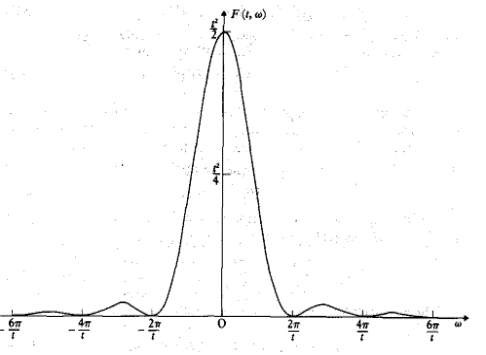
\includegraphics[scale=0.4]{ch2/image1}
	\captionof{figure}{ }
	\end{wrapfigure}
Ci-contre, une représentation de $F(t,\tilde{\omega})$. Il ne s'agit pas d'un delta de \textsc{Dirac}.
Par contre, sous l'approximation du temps long, la largeur du pulse devient suffisamment mince que
pour considérer que c'est le cas
\begin{equation}
F(t \rightarrow \infty, \tilde{\omega}) \sim \pi t \; \delta(\tilde{\omega})
\end{equation}
Revenons au calcul précédent en utilisant ce résultat pour l'intégration sur tous les
$\tilde{\omega}$
\begin{equation}
  \vert c_b^{(1)} (t) \vert ^2 = 
\frac{1}{2} \left( \frac{e}{m} \right) ^2
A_0^2 (\omega_{ba}) 
     \vert M_{ba} (\omega_{ba}) \vert ^2 \; 
\underbrace{\int_{-\infty}^{+\infty}
F(t, \tilde{\omega}) d \tilde{\omega}}_{\pi t}
\end{equation}
On trouve alors que la probabilité augmente \textbf{linéairement} avec $t$ \\

\cadre{\begin{equation}
\vert c_b^{(1)} (t) \vert ^2 = \frac{\pi}{2}
 \left[ \frac{e A_0 (\omega_{ba})}{m} \right] ^2
    \vert M_{ba} (\omega_{ba}) \vert ^2 \; t
\end{equation}}\ \\

Il s'agit d'une nouvelle condition de résonance nous informant sur le fait que $\omega$ doit
être proche de $\omega_{ba}$.\footnote{A vérifier.}

\section{Absorption et émission stimulées}
La probabilité d'\textbf{absorption} s'obtient en dérivant temporellement le module carré calculé 
ci-dessus
\begin{equation}
W_{b \leftarrow a} =
\frac{d}{dt} \vert c_b^{(1)} (t) \vert ^2 =
\frac{\pi}{2} \left[ \frac{e A_0 (\omega_{ba}) }{m} \right] ^2 
\vert M_{ba} (\omega_{ba}) \vert ^2
\end{equation}
En reprenant le lien entre $A_0$ est $I$ (en début de chapitre, avec le vecteur de \textsc{Poynting})
\begin{equation}
W_{b \leftarrow a} =\frac{4 \pi ^2}{m^2 c} \left( \frac{e^2}{4 \pi \epsilon_0 } \right)
\frac{I( \omega_{ba}) }{\omega_{ba}^2 } \vert M_{ba} (\omega_{ba}) \vert ^2
\end{equation}
Cette probabilité sera  non nulle lorsque l'élément matriciel $M_{ba}$ est nul nul. Ceci met en 
évidence la quantification de la matière par l'atome d'hydrogène. L'interaction lumière-matière sera
traitée de façon semi-classique. \\

Il existe un effet symétrique inverse à celui-ci : $\tilde W_{b\leftarrow a}=W_{b\leftarrow a}$. Ce
phénomène est l'\textbf{émission stimulée} dont la probabilité est donné par
\begin{equation}
\tilde{W}_{a \leftarrow b} = \frac{4 \pi ^2}{m^2 c} \left( \frac{e^2}{4 \pi \epsilon_0 } \right)
\frac{I( \omega_{ba}) }{\omega_{ba}^2 } \vert \tilde{M}_{ab} (\omega_{ba}) \vert ^2
\end{equation}
En définissant l'élément de matrice
\begin{equation}
\tilde{M}_{ab} = \langle \psi_a \vert e^{-i {\bf k} \cdot {\bf r} }
  \hat{  \mbox{\boldmath $ \epsilon $}} \cdot \mbox{\boldmath $ \nabla $} \vert \psi_b \rangle
\end{equation}
En comparant cet élément matriciel au précédent, c'est sans surprise que l'on retrouve
\begin{equation}
\tilde{M}_{ab} = - M_{ba}^{\ast} \Rightarrow \tilde{W}_{a \leftarrow b} = W_{b \leftarrow a}
\end{equation}
La seule différence par rapport au cas précédent se situe donc dans l'élément de matrice. Les 
populations $a$ et $b$ ne seront pas peuplées de la même façon. Selon \textsc{Boltzmann}, la 
population dépend de l'énergie ($N\propto g_ie^{-E/kT}$). Si l'on tient compte de ce facteur 
de proportionnalité, il y a plus de change d'observer une absorption qu'une émission stimulé. Ceci
n'est évidemment pas le cas dans des dispositifs comme les \textit{laser} où il y a eu inversion 
de la population, mais rappelons que cette situation ne décrit pas un équilibre thermodynamique.



\section{Le photon QED et l'émission spontanée}
Nous avons jusqu'ici suivi une approche semi-classique. En passant par le théorie quantique des 
champs, nous allons essayer d'estimer l'erreur faite (section informative si j'ai bien compris). 

\subsection{Absorption d'un photon à partir d'un état à $N$ photons}
En quantifiant le champ électrique, on retrouve un potentiel vecteur ayant exactement la même forme
que précédemment
\begin{equation}
  {\bf A}_1 = 
  \hat{  \mbox{\boldmath $ \epsilon $}}
\left[  \frac{2 N(\omega) \hbar}{ V \epsilon_0 \omega}
  \right] ^{1/2} \frac{1}{2}
  \exp [ i ( {\bf k} \cdot {\bf r} - \omega t 
+ \delta_{\omega} )  ] 
\end{equation}
On trouve alors la même expression qu'avant, la QED n'apporte rien ici
\begin{equation}
W_{b \leftarrow a} ^{QED} = 
W_{b \leftarrow a} 
= \frac{4 \pi ^2}{m^2 c} \left( \frac{e^2}{4 \pi \epsilon_0 } \right)
\frac{I( \omega_{ba}) }{\omega_{ba}^2 } \vert M_{ba} \vert ^2
\end{equation}


\subsection{Création d'un photon}
Par de chance cette fois-ci, le potentiel vecteur n'est pas totalement similaire
\begin{equation}
  {\bf A}_2 = 
  \hat{  \mbox{\boldmath $ \epsilon $}}
\left[ \frac{ 2(  N(\omega)+1) \hbar}{ V \epsilon_0 \omega}
  \right] ^{1/2} \frac{1}{2}
   \exp [ -i ( {\bf k} \cdot {\bf r} 
- \omega t + \delta_{\omega} ) ]
\end{equation}
La différence, c'est ce +1. Il s'agit du photon qui manque à la théorie semi-classique. Dès lors
\begin{equation}
\tilde{W}_{a \leftarrow b}^{QED} =
 \frac{4 \pi ^2}{m^2 } \left( \frac{e^2}{4 \pi \epsilon_0 } \right)
\frac{( N (\omega_{ba}) + 1) \hbar }{V \omega_{ba} } \vert M_{ba} \vert ^2
  \delta(\omega - \omega_{ba} )
\end{equation}
Rassurons-nous, c'est quasi-négligeable ($ N (\omega_{ba}) + 1 \approx N (\omega_{ba})$). On peut
alors souvent écrire, en approximation
\begin{equation}
\tilde{W}_{a \leftarrow b}^{QED} \approx
\tilde{W}_{a \leftarrow b} =  
\frac{4 \pi ^2}{m^2 c} \left( \frac{e^2}{4 \pi \epsilon_0 } \right)
\frac{I( \omega_{ba}) }{\omega_{ba}^2 } \vert \tilde{M}_{ab} \vert ^2
\end{equation}
Ceci signifie qu'un atome dans un état excité, même dans le vide le plus total, peut émettre un
photon grâce à ce "+1" (en se désexcitant).\\

En résumé, nous pouvons dire que
\begin{equation}
\left\{\begin{array}{ll}
\mbox{semi-classique:} & N(\omega_{ba}) \\
\mbox{QED:} & N(\omega_{ba}) + 1
\end{array} \right.
\end{equation}
Reprenons la précédente expression débarrassée du $N(\omega)$, soit juste le terme "+1" que nous
avions manqué dans l'approche semi-classique. Il s'agit de la \textit{probabilité d'émission
\textbf{spontanée}}
\begin{equation}
W_{a \leftarrow b}^s =
 \frac{4 \pi ^2}{m^2 } \left( \frac{e^2}{4 \pi \epsilon_0 } \right)
\frac{\hbar }{V \omega_{ba} } \vert M_{ba} \vert ^2
  \delta(\omega - \omega_{ba} )
\end{equation}
Afin d'interpréter ce terme, nous allons faire un petit détour par la \textit{Règle d'Or de Fermi}\\

\cadre{
$$\rho_b(E) \equiv~\mbox{densit\'e de niveaux}
\Rightarrow
P_{ba}(t) = \frac{2 \pi}{\hbar} \vert H'_{ba} \vert ^2
\rho_b(E) t$$
$$\mbox{prob. transition par unit\'e de tps}:~
W_{b \leftarrow a} = dP_{ba}/dt $$
$$W_{b \leftarrow a} = \frac{2 \pi}{\hbar} \vert H'_{ba} \vert ^2
\rho_b(E)$$
Il s'agit de la probabilité de passage d'un état $a$ vers un état $b$ où le passage se fait d'un
état d'énergie discret vers un état continu.}\ \\

Évaluons la densité d'états pour le photon final. Après un peu de physique du solide (en admettant
le concept de cavité de résonance)\footnote{\textit{Ceci est donné pour faire plaisir mais n'est
pas matière d'examen}}
\begin{equation}
dn_x \; dn_y \; dn_z = \left( \frac{L}{2 \pi}  \right) ^3
dk_x \; dk_y \; dk_z
 = \left( \frac{L}{2 \pi}  \right) ^3
k^2 \; dk \; d\Omega
\end{equation}
Sachant que $V=L^3$ et $w=kc$, on peut obtenir le nombre de photon compris entre $\omega$ et 
$w+d\omega$ dans un angle solide $d\Omega$
\begin{equation}
\rho_a (\omega) d \omega d \Omega = \frac{V}{(2 \pi)^3}
\frac{\omega^2}{c^3} d \omega d \Omega 
\end{equation}
En reprenant l'expression de l'émission spontanée $W^s$ et en y insérant la règle d'or de Fermi, 
on trouve
\begin{equation}
W_{a \leftarrow b}^s(\theta,\phi) d \Omega = 
\frac{\hbar}{ 2 \pi m^2 c^3} \left( \frac{e^2}{4 \pi \epsilon_0 } \right)
 \omega_{ba} \vert M_{ba} (\omega_{ba}) \vert ^2
d \Omega
\end{equation}
Ceci n'est rien autre que la probabilité d'émission \textbf{spontanée} par unité de temps d'un photon
de fréquence $\omega_{ba}$ dans une direction particulière à l'intérieur d'un angle solide $d\Omega$.


\section{L'approximation dipolaire électrique}
Lorsqu'un atome excité se désexcite par l'émission d'un photon, rien ne dit que celui-ci sera
polarisé et de même pour sa direction. Il faut alors intégrer sur tous les angles d'émission tout
en sommant sur les deux états de polarisation
\begin{equation}
W_{a \leftarrow b}^s = \frac{\hbar}{ 2 \pi m^2 c^3} \left( \frac{e^2}{4 \pi \epsilon_0 } \right)
\int d\Omega \sum_{\lambda = 1}^2 \omega_{ba} \vert M^{\lambda}_{ba} (\omega_{ba}) \vert ^2
\end{equation}
Outre cette dépendance fréquentielle, on retrouve le même élément de matrice couplant $a$ et $b$. La
question est maintenant de savoir ce que vaut cet élément de matrice et pour ça, nous allons faire
l'\textit{approximation dipolaire électrique (E1)}. Considérons le développement en série
\begin{equation}
e^{i {\bf k} \cdot {\bf r} } = 1 + (i {\bf k} \cdot {\bf r} ) + \frac{1}{2!} 
  ( i {\bf k} \cdot {\bf r} ) ^2 + \ldots
\end{equation}
Si l'on se trouve dans le cas des transitions optiques, $ \leq  1~\mbox{\AA~et }~k = 2 \pi / \lambda
\approx 10^5~\mbox{cm}^{-1}$. Il en vient que $(kr)\ll 1$. On peut approximer l'exponentielle 
à un dans ce régime la
\begin{equation}
e^{i {\bf k} \cdot {\bf r} } \approx  1  \Rightarrow
M_{ba} = \hat{  \mbox{\boldmath $ \epsilon $}} \cdot \langle \psi_b \vert
\mbox{\boldmath $ \nabla $} \vert \psi_a \rangle
\end{equation}
Il faudra alors juste calculer les éléments de matrice de l'opérateur gradient. Connaissant les 
deux relations suivantes reliant l'impulsion et la vitesse, on peut ré-écrire cet élément de 
matrice
\begin{equation}
\left.
\begin{array}{l}
{\bf p} = m \dot{{\bf r}} = -i \hbar \mbox{\boldmath $ \nabla $} \\
\dot{{\bf r}}  = \frac{1}{i \hbar} [ {\bf r}, H_0 ] \end{array}
\right\} \Rightarrow
M_{ba} = - \frac{m \omega_{ba}}{\hbar} \hat{  \mbox{\boldmath $ \epsilon $}} \cdot 
\langle \psi_b \vert {\bf r} \vert \psi_a \rangle
\end{equation}
Cette forme permet de comprendre le nom de l'approximation : on voit apparaître la position 
moyenne qui, multipliée à la charge, donne le \textit{moment dipolaire}. Sachant que
$ $, on peut écrire
\begin{equation}
W^{E1}_{b \leftarrow a} = \frac{4 \pi^2}{c \hbar^2} \left( \frac{1}{4 \pi \epsilon_0 } \right)
 I(w_{ba}) \vert  \hat{  \mbox{\boldmath $ \epsilon $}} \cdot 
 \mbox{\boldmath $ \mu $}_{ba} \vert ^2
\end{equation}
En faisant apparaître $\vec\mu$ via le formalisme position, la probabilité $E1$ permet de comprendre
le passage de $a$ à $b$ (ou l'inverse) où apparaît le moment dipolaire entre les deux états. On peut
alors trouver la radiation isotropique non polarisée pour l'absorption
\begin{equation}
W^{E1}_{b \leftarrow a} = \frac{4 \pi^2}{3 c \hbar^2} \left( \frac{1}{4 \pi \epsilon_0 } \right)
 I(w_{ba}) \vert  
 \mbox{\boldmath $ \mu $}_{ba} \vert ^2
\end{equation}
Et de même pour l'émission spontanée
\begin{equation}
W_{a \leftarrow b}^{E1,s} = \frac{4}{3 \hbar c^3} \left( \frac{1}{4 \pi \epsilon_0} \right)
  \omega_{b a}^3 \vert  \mbox{\boldmath $ \mu $}_{ba} \vert ^2
\end{equation}
On remarque que plus la différence entre $a$ et $b$ est grande, plus la probabilité de transition
est grande : c'est le \textit{comportement suicidaire de l'électron}.\\


	\begin{wrapfigure}[8]{r}{5cm}
	\vspace{-5mm}
	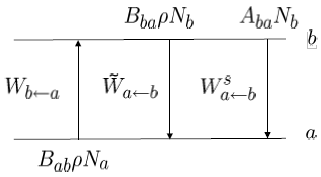
\includegraphics[scale=0.6]{ch2/image2}
	\captionof{figure}{ }
	\end{wrapfigure}
On peut (et en on parlera d'avantage dans la section suivante) faire le lien avec les coefficients
d'\textsc{Einstein}. Commentons les transitions ci-contre. Pour que la première flèche existe, il
faut que $N_a$ existe, mais également une densité de radiation $\rho$. Le coefficient $B_{ab}$ n'est
autre que le coefficient de proportionnalité donnant une probabilité. Il existe également le 
phénomène symétrique (seconde flèche) : il faut ici que $N_b$ soit peuplé et qu'il y ai une certaine
densité de radiations. La troisième flèche (émission spontanée) peut elle se produire sans radiation
à condition que le niveau $b$ soit peuplé.


\section{Lien avec les coefficients d'Einstein}
Écrivons l'équation cinétique du niveau $a$. La transition $a\to b$ dépeuple $a$ tandis que
la $b\to a$ le repeuple
\begin{equation}
\frac{dN_a}{dt} = - \frac{dN_b}{dt} =
- B_{ab} \rho(\omega_{ba}) N_a + B_{ba} \rho(\omega_{ba}) N_b
 + A_{ba} N_b
\end{equation}
A l'équilibre, $\frac{dN_a}{dt} = \frac{dN_b}{dt} = 0$. On peut en tirer un expression de $\rho$
\begin{equation}
\rho(\omega_{ba}) = 
\frac{A_{ba} }{B_{ab} (N_a/N_b) - B_{ba}}
\end{equation}
L'équation de \textsc{Boltzmann} (en oubliant les facteurs de dégénérescence) permet de déterminer
l'évolution du rapport $N_a/N_b$
\begin{equation}
\frac{N_a}{N_b} = e^{-(E_a - E_b)/kT} = e^{\hbar \omega_{ba} /kT}
\end{equation}
De son côté, \textsc{Planck} a proposé un expression pour la densité d'un corps noir
\begin{equation}
\rho(\omega_{ba})
= \frac{\hbar \omega_{ba}^3}{\pi^2 c^3}
\frac{1}{e^{\hbar \omega_{ba} /kT} -1  }
\end{equation}
\textsc{Einstein} avait les précédentes équations sous la main.  Il a remarqué - avec en plus 
l'équation de \textsc{Boltzmann} à disposition - que l'égalité entre son $\rho$ et celui trouvé par
\textsc{Planck} est vérifiée si les conditions si les conditions suivantes sont respectées
\begin{equation}
\left\{
\begin{array}{l}
B_{ab} = B_{ba} \\
A_{ba} = \frac{\hbar \omega_{ba}^3}{\pi^2 c^3} \; B_{ba}
\end{array} \right. \quad\Leftrightarrow\quad
 \left\{ \begin{array}{l}
B_{ab} = \frac{W_{b \leftarrow a}}{\rho} \\
A_{ba} = W^s_{a \leftarrow b}
\end{array} \right.
\end{equation}
\textsc{Interprétation manquante} (au pire, cf. \textit{Physique des lasers}).

\section{Spectre des atomes hydrogénoïdes}
Maintenant que nous avons établi la forme de l'élément matriciel, il serait intéressant de comprendre
comment celui-ci couple les états $n=2$ et $n=3$ par exemple. Pour se faire, reprenons la probabilité
de transition d'émission stimulée et spontanée($s$)
\begin{equation}
\begin{array}{ll}
W^{E1}_{b \leftarrow a} &\DS= \frac{4 \pi^2}{c \hbar^2} \left( \frac{e^2}{4 \pi \epsilon_0 } \right)
 I(w_{ba}) \vert  \hat{  \mbox{\boldmath $ \epsilon $}} \cdot 
{\bf  r}_{ba} \vert ^2\vspace{2mm}\\
W_{a \leftarrow b}^{E1,s}(\theta, \phi) \; d \Omega &\DS= 
\frac{1}{2 \pi \hbar c^3} \left( \frac{e^2}{4 \pi \epsilon_0} \right)
  \omega_{b a}^3
\vert  \hat{  \mbox{\boldmath $ \epsilon $}} \cdot 
{\bf  r}_{ba} \vert ^2 d \Omega
\end{array}
\end{equation}
Exprimons le vecteur polarisation $\hat{\vec{\epsilon}}$ en composantes sphériques
\begin{equation}
\left\{
\begin{array}{ll }
\epsilon^{(1)}_{+1}  & = - \frac{1}{\sqrt{2}} 
 \left( \hat{\epsilon}_x + i  \hat{\epsilon}_y \right) \\
\epsilon^{(1)}_{0}  & =  \hat{\epsilon}_z \\
\epsilon^{(1)}_{-1}  & = + \frac{1}{\sqrt{2}}
 \left(  \hat{\epsilon}_x - i  \hat{\epsilon}_y \right)
\end{array} \right.
\end{equation}
En faisant de même pour le vecteur $\vec{r}$
\begin{equation}
\left\{
\begin{array}{ll }
r^{(1)}_{+1}  & = - \frac{1}{\sqrt{2}} \left( x + i y \right) \\
r^{(1)}_{0}  & = z \\
r^{(1)}_{-1}  & = + \frac{1}{\sqrt{2}} \left( x - i y \right)
\end{array} \right.
\end{equation}
Ceci forme un tenseur sphérique irréductible d'ordre 1 (se transforme comme un vecteur par
rotation). A partir de deux tenseur, il est possible d'en tirer un tenseur scalaire. Il faut
pour cela faire un produit tensoriel des deux OTI
\begin{equation}
\left[ {\bf T}^{(k_1)} \times {\bf W}^{(k_2)} \right]^{(K)}_Q \equiv
\sum_{q_1,q_2} C(k_1k_2q_1q_2;KQ) \; T^{(k_1)}_{q_1} W^{(k_2)}_{q_2}
\end{equation}
En couplant des tenseurs sphériques irréductibles, il est possible de créer un tenseur irréductible
scalaire.

\subsubsection*{Parenthèse : symboles $3-j$}
Pour se faciliter la vie, on introduit les symboles $3-j$. Pour comprendre leur utilité, repartons
des coefficients de Clebsch-Gordon
\begin{equation}
C(j_1 j_2 m_1 m_2; J M) 
= ( j_1 j_2 m_1 m_2 \vert j_1 j_2 J M)= ( j_1 j_2 m_1 m_2 \vert  J M) 
= ( j_1 m_1 j_2 m_2 \vert  J M)
\end{equation}
Par \textbf{définition} des \textit{symboles $3-j$}
\begin{equation}
( j_1 j_2 m_1 m_2 \vert j_1 j_2 J M)
\equiv
(-1)^{j_1 - j_2 + M} [ J ]^{1/2} 
\left( \begin{array}{ccc} j_1 & j_2 & J \\ m_1 & m_2 & -M \end{array} 
\right) 
\end{equation}
L'utilité de ces symboles se trouve dans les propriétés de ceux-ci
\begin{equation}
\left( 
\begin{array}{ccc} j_1 & j_2 & j_3 \\ m_1 & m_2 & m_3 \end{array} 
\right) 
= 
\left( 
\begin{array}{ccc} j_2 & j_3 & j_1 \\ m_2 & m_3 & m_1 \end{array} 
\right)= (-1)^{j_1 + j_2 + j_3}
\left( 
\begin{array}{ccc} j_2 & j_1 & j_3 \\ m_2 & m_1 & m_3 \end{array} 
\right)
\end{equation}
Ceux-ci sont non nuls si
\begin{equation}
 \neq 0 \Rightarrow \left\{
\begin{array}{l}
\delta(j_1,j_2,j_3) \\
m_1 + m_2 + m_3 = 0
\end{array}  \right.
\end{equation}
Ce qui constitue une puissante règle de sélection.

\subsection{Produit scalaire de 2 OTI}
Construisons le produit scalaire entre deux OTI. Pour se faire, évaluons le produit entre deux
tenseurs suivant\footnote{Je n'ai pas de notes sur ce slide (20), si quelqu'un peut compléter}
\begin{equation}
\left[ T^{(k)} \times W^{(k)} \right]^{(0)}_0 \equiv
\sum_{q} 
\left( \begin{array}{ccc} k & k & 0 \\ -q & q & 0 \end{array} 
\right)  \; T^{(k)}_{-q} W^{(k)}_{q}
= (-1)^k [k]^{-1/2} \sum_q (-1)^q \; T^{(k)}_{-q} W^{(k)}_{q}
\end{equation}
On en tire l'expression du produit scalaire tensoriel\\

\cadre{
\begin{equation}
Q \equiv T^{(k)} \cdot W^{(k)} \equiv
\sum_q (-1)^q \; T^{(k)}_{-q} W^{(k)}_{q}
\end{equation}}\ \\

Nous avons comme probabilité de transition
\begin{equation}
W^{E1}_{b \leftarrow a} = \frac{4 \pi^2}{c \hbar^2} \left( \frac{e^2}{4 \pi \epsilon_0 } \right)
 I(w_{ba}) \vert  \hat{  \mbox{\boldmath $ \epsilon $}} \cdot 
{\bf  r}_{ba} \vert ^2
\end{equation}
Développons le produit scalaire se trouvant dans le module carré
\begin{equation}
\begin{array}{ll}
  \hat{  \mbox{\boldmath $ \epsilon $}} \cdot 
{\bf  r}_{ba}
&\DS= - \epsilon^{(1)}_{-1} \left( r^{(1)}_{+1} \right)_{ba} 
+ \epsilon^{(1)}_{0} \left(  r^{(1)}_{0} \right)_{ba}
- \epsilon^{(1)}_{+1}\left(  r^{(1)}_{-1} \right)_{ba}\vspace{2mm}\\
&\DS= +  \epsilon^{(1)\ast}_{+1}  \left( r^{(1)}_{+1} \right)_{ba} 
+  \epsilon^{(1)\ast}_{0}  \left(  r^{(1)}_{0} \right)_{ba}
+  \epsilon^{(1)\ast }_{-1}  \left(  r^{(1)}_{-1} \right)_{ba}\vspace{2mm}\\
&\DS= \sum_q \; \epsilon^{(1)\ast}_q I^q_{n'l'm';nlm}
\end{array}
\end{equation}
Dans l'atome d'hydrogène, $a$ et $n$ ne sont finalement qu'un \textit{set} de nombres quantiques.
Continuons en explicitant $I^q_{n'l'm';nlm}$
\begin{equation}
\begin{array}{ll}
I^q_{n'l'm';nlm} &\DS=  \sqrt{\frac{4 \pi}{3}} \int_0 ^\infty
\; dr \; r^3 R_{n'l'}(r)^\ast  R_{nl}(r)\times \int_0^{2 \pi} \int_0^{\pi}
Y^\ast_{l'm'} Y_{1q} Y_{lm} \sin \theta d\theta d\phi\vspace{2mm}\\
&\DS= \langle l' m' \vert C^{(1)}_q \vert l m  \rangle \int_0 ^\infty
\; dr \; r^3 R_{n'l'}(r)  R_{nl}(r)
\end{array}
\end{equation}
où l'on voit apparaître les harmoniques sphériques de l'opérateur. Explicitons cette fois 
$\langle l' m' \vert C^{(1)}_q \vert l m \rangle$
\begin{equation}
\langle l' m' \vert C^{(1)}_q \vert l m \rangle
= \sqrt{\frac{4 \pi}{3}} \int_0^{2 \pi} \int_0^{\pi}
Y^\ast_{l'm'} Y_{1q} Y_{lm} \sin \theta d\theta d\phi
= (-1)^{-m'} [l',l]^{1/2}
\left( \begin{array}{ccc} l' & 1 & l \\ 0 & 0 & 0 \end{array} \right)
\left( \begin{array}{ccc} l' & 1 & l \\ -m' & q & m \end{array} \right)
\end{equation}
Grâce à la propriété des coefficients $3-j$ énoncée ci-dessus, on en tire la \textbf{forte} 
règle de sélection suivante :\\

\cadre{\begin{equation}
 \neq 0 \Rightarrow \left\{
\begin{array}{l}
\delta(l',1,l) \\
(l' +1 + l)~\mbox{pair} \end{array} \right\} 
\Rightarrow \Delta l = l' - l = \pm 1
\end{equation}}\ \\

Le nombre quantique $l$ ne peut varier que d'au maximum \textbf{une} unité lors d'une transition.
On obtient finalement quelque chose de simple, à géométrie sphérique
\begin{equation}
-m' + q + m = 0 \Rightarrow
\left\{ \begin{array}{ll}
m' = m \; \; (\Delta m = 0) & \mbox{si}~q = 0 \\
m' = m \pm 1 \; \; (\Delta m = \pm 1) &\mbox{si}~q = \pm 1
\end{array} \right.
\end{equation}\ \\

A l'aide de l'explicitation de $\langle l' m' \vert C^{(1)}_q \vert l m \rangle$, on peut 
ré-écrire $I^q_{n'l'm';nlm}$
\begin{equation}
I^q_{n'l'm';nlm} =  \sqrt{\frac{4 \pi}{3}} \int_0 ^\infty
\; dr \; r^3 R_{n'l'}(r)^\ast  R_{nl}(r)\times \int_0^{2 \pi} \int_0^{\pi}
Y^\ast_{l'm'} Y_{1q} Y_{lm} \sin \theta d\theta d\phi
\end{equation}


\subsection{Lien de la règle de sélection $\Delta l = \pm 1$ avec la parité}
Nous avons
\begin{equation}
\phi_{ n l m }(r, \theta, \phi) = R_{nl} (r) Y_{lm} (\theta, \phi)
\end{equation}
A l'aide de l'opérateur parité
\begin{equation}
\hat{I} \phi_{ n l m }({\bf r}) = 
\hat{I} R_{nl} (r) Y_{lm} (\theta, \phi)
\equiv 
\phi_{ n l m }( - {\bf r})=
R_{nl} (r) Y_{lm} (\pi - \theta, \phi + \pi)
=  (-1)^l R_{nl} (r) Y_{lm} (\theta, \phi)
\end{equation}
En en tire que
\begin{equation}
\begin{array}{ll}
I^q_{n'l'm';nlm} &\DS=  (-1)^{l' + 1 + l}  I^q_{n'l'm';nlm}\\
&\DS \neq 0 ~\mbox{si}~(l' +1 + l)~\mbox{pair} 
\end{array}
\end{equation}
En résumé, l'inversion ne touche que la partie sphérique. Si $l$ est pair la parité sera impaire
et paire inversement. On en déduit qu'une\textbf{transition E1 ne peut relier que des états de
parité différentes}. La règle $\Delta l=\pm1$ est la \textit{règle de }\textsc{Laporte}. Le
\textit{slide 23} représente les transitions à l'aide de cette règle de sélection tandis que 
le \textit{slide 24} les classe par parité.


\section{Force de raie, force d'oscillateur et temps de vie}
Le théorème de \textsc{Wigner-Eckart} est apprécié pour les règles de sommes extraordinaires
des $3-j$ mais aussi pour ses règles de sélection.\\

\theor{\textsc{Wigner-Eckart}\ 
\begin{equation}
\langle \alpha j m \vert T^{(k)}_q \vert \alpha' j' m' \rangle
= (-1)^{j-m} \left( \begin{array}{ccc}
j  &  k  &  j'  \\ -m  &  q  &  m' \end{array} \right) 
\langle \alpha j \Vert {\bf T}^{(k)} \Vert \alpha' j' \rangle
\end{equation}}\ \\

Chaque élément de matrice peut s'écrire comme un élément de matrice réduit multiplié par un
$3-j$. Ré-écrivons alors l'élément de matrice qui nous intéresse sous cette forme
\begin{equation}
 \langle l m_l \vert C^{(1)}_q \vert l'm_l' \rangle =
(-1)^{l-m_l} \left( \begin{array}{ccc}
l  &  1  &  l'  \\ -m_l  &  q  &  m_l' \end{array} \right) 
\langle  l \Vert {\bf C}^{(1)} \Vert l' \rangle
\end{equation}
L'élément de matrice réduit s'écrit
\begin{equation}
\langle  l \Vert {\bf C}^{(1)} \Vert l' \rangle
= (-1)^l [l,l']^{1/2} \left( \begin{array}{ccc}
l  &  1  &  l'  \\ 0  &  0 &  0 \end{array} \right)
\end{equation}
Énonçons la fabuleuse \textbf{règle de somme}
\begin{equation}
\sum_{mm'}  \vert
\langle \alpha j m \vert T^{(k)}_q \vert \alpha' j' m' \rangle \vert ^2
= \vert \langle \alpha j \Vert {\bf T}^{(k)} \Vert \alpha' j' \rangle \vert ^2 
\sum_{mm'} \left( \begin{array}{ccc}
j  &  k  &  j'  \\ -m  &  q  &  m' \end{array} \right) ^2 
=  \frac{1}{2k+1} \vert \langle \alpha j \Vert {\bf T}^{(k)} \Vert \alpha' j' \rangle \vert ^2
\end{equation}


\subsection{Force de raie et force d'oscillateur}
Appliquons la règle de somme et utilisons une notation plus efficace
\begin{equation}
S(\alpha J, \alpha' J' ) = \sum_{MM'q} \vert \langle \alpha JM \vert \mu^{(1)}_q  \vert \alpha J' M' \rangle \vert^2= 
\vert \langle \alpha J \Vert 
\mbox{\boldmath $ \mu $}^{(1)} \Vert \alpha J' \rangle \vert^2
\end{equation}
Suite au cours de demain!

\iffalse
unité atomique de moment dipolaire au carré. C'est (e*a0)^2 l'unité de ça

303.7 : nombre quand S exprime en u.a., quand lamda est en 1. il faut... pour calculer un nombre sans dimension

nombre sans dim qui va introduire la force d'oscillateur. EN injectant çala dedans on trouve 1. g_k c'est facteur de dégen
\fi






















